%%%%%%%%%%%%%%%%%%%%%%%%%%%%%%%%%%%%%%%%%%%%%
% Compile: XeLaTeX BibTeX XeLaTeX XeLaTeX
%%%%%%%%%%%%%%%%%%%%%%%%%%%%%%%%%%%%%%%%%%%%%

\documentclass[10pt, paper=a4, abstracton]{scrartcl}

%%%%%%%%%%%%%PACKAGES%%%%%%%%%%%%%

\usepackage[ngerman, english]{babel}

\usepackage{libertine}

\usepackage{blindtext}

\usepackage{graphicx}

%%%%%%%%%%%%%COMMANDS%%%%%%%%%%%%

%%%%%%%%%%%%%META DATA%%%%%%%%%%%%
\author{Sebastian Nordhoff \and Antonio Machicao y Priemer}
\title{\LaTeX\ for Linguists}
\subtitle{My first \TeX\ document}
\date{July 29, 2019}

%%%%%%%%%%%%END PREAMBLE%%%%%%%%%%%

%%%%%%%%%%BEGIN DOCUMENT%%%%%%%%%%%

\begin{document}

\maketitle

\tableofcontents

\newpage

\begin{abstract}
	An abstract is a brief summary of a research article, thesis, or any in-depth 
	analysis of a particular subject and is often used to help the reader quickly 
	ascertain the paper's purpose.\par 
	When used, an abstract always appears at the beginning of a manuscript, acting 
	as the point-of-entry for any given academic paper. 
\end{abstract}


\section[Headlines and paragraphs]{Playing with headlines and paragraphs}

This is my first \LaTeX\ file. 

This an example with a word in \textbf{bold}. This an example with a word in \textit{italics}.

\begin{center}
	This sentence is centered.
\end{center}

This sentence is not centered. 

This sentence has a {\Huge huge} word. This sentence is in normal size.


\subsection[First subsection]{My first subsection}

This is a sample text. The only purpose of this text is to show how to work with \LaTeX . It is not necessary that this text has any meaning. It should only show some properties of the system we are using. This is a sample text. The only purpose of this text is to show how to work with \LaTeX . It is not necessary that this text has any meaning. It should only show some properties of the system we are using. 


\subsubsection[First subsubsection]{My first subsubsection}

This is a sample text. The only purpose of this text is to show how to work with \LaTeX . It is not necessary that this text has any meaning. It should only show some properties of the system we are using. This is a sample text. The only purpose of this text is to show how to work with \LaTeX . It is not necessary that this text has any meaning. It should only show some properties of the system we are using. 


\subsection[Second subsection]{My second subsection}

This is a sample text. The only purpose of this text is to show how to work with \LaTeX . It is not necessary that this text has any meaning. It should only show some properties of the system we are using. This is a sample text. The only purpose of this text is to show how to work with \LaTeX . It is not necessary that this text has any meaning. It should only show some properties of the system we are using. 


\subsubsection[Second subsubsection]{My second subsubsection}

This is a sample text. The only purpose of this text is to show how to work with \LaTeX . It is not necessary that this text has any meaning. It should only show some properties of the system we are using. This is a sample text. The only purpose of this text is to show how to work with \LaTeX . It is not necessary that this text has any meaning. It should only show some properties of the system we are using. 


\subsection[Paragraphs and line brakes]{Playing with paragraphs and line brakes}

This is a sample text. The only purpose of this text is to show how to work with \LaTeX . It is not necessary that this text has any meaning. It should only show some properties of the system we are using. \par 

This is a sample text. The only purpose of this text is to show how to work with \LaTeX . It is not necessary that this text has any meaning. It should only show some properties of the system we are using. 

This is a sample text. The only purpose of this text is to show how to work with \LaTeX . It is not necessary that this text has any meaning. It should only show some properties of the system we are using. 

\noindent This text is \textbf{not indented}. This is a sample text. The only purpose of this text is to show how to work with \LaTeX . It is not necessary that this text has any meaning. It should only show some properties of the system we are using. \\
This text is \textbf{not indented}. This is a sample text. The only purpose of this text is to show how to work with \LaTeX . It is not necessary that this text has any meaning. It should only show some properties of the system we are using. 

This is a sample text. The only purpose of this text is to show how to work with \LaTeX . It is not necessary that this text has any meaning. It should only show some properties of the system we are using. 


\paragraph[First paragraph]{My first paragraph}

This is a sample text. The only purpose of this text is to show how to work with \LaTeX . It is not necessary that this text has any meaning. It should only show some properties of the system we are using. 


\subparagraph[First subparagraph]{My first subparagraph}

This is a sample text. The only purpose of this text is to show how to work with \LaTeX . It is not necessary that this text has any meaning. It should only show some properties of the system we are using. 


\section[Footnotes]{Playing with footnotes}

This is a sample text. The only purpose of this text%
%
\footnote{A text (literary theory) is any object that can be read.} %
%
is to show how to work with footnotes in \LaTeX .%
%
\footnote{\LaTeX\ is a document preparation system.} %
%
It is not necessary that this text has any meaning. It should only show some properties of the system we are using. 


\section{Special characters}

Here you can practice some commands for accents: \"U \"E \"y \"o \'i \`e \=a \ss{} \^u \~n \v{c} 


\noindent This is a sample list of special characters: \textbackslash\ \textasciitilde\ \textasciicircum\ 
\textgreater\ $<$ \textbar \#  \$  \&  \_  \{  \}  \%


\section{Spacing \& line breaks}

  Write this sentence with five blanks before the first word in this sentence. Put five blanks after the following German word: \textit{Mu{\ss}e}      and put one line break after the following Spanish word: \textit{ni\~no}
  and now, put one empty line after the last word of this sentence.
  
  To finish, put 9 empty lines after the end of this sentence.
  
  
  
  
  
  
  
  
  This is a sample text. The only purpose of this text is to show how to work with \LaTeX . It is not necessary that this text has any meaning. It should only show some properties of the system we are using.


\section{Commenting out}


\subsection{Finding the error}

Copy the following two paragraphs into your document and find the error in the code by commenting out the paragraphs and parts of the paragraphs.


This is a sample text. The only purpose of this text is to show how to work with \LaTeX . It is not necessary that this text has any meaning. It should only show some properties of the system we are using. This is a sample text. The only purpose of this text is to show how to work with \LaTeX . It is not necessary that this text has any meaning. It should only show some properties of the system we are using. This is a sample text. The only purpose of this text is to show how to work with \LaTeX . It is not necessary that this text has any meaning. It should only show some properties of the system we are using. This is a sample text. The only purpose of this text is to show how to work with \LaTeX . It is not necessary that this text has any meaning. It should only show some properties of the system we are using. This is a sample text. The only purpose of this text is to show how to work with \LaTeX . It is not necessary that this text has any meaning. It should only show some properties of the system we are using. This is a sample text. The only purpose of this text is to show how to work with \LaTeX . It is not necessary that this text has any meaning. It should only show some properties of the system we are using. This is a sample text. The only purpose of this text is to show how to work with \LaTeX . It is not necessary that this text has any meaning. It should only show some properties of the system we are using. This is a sample text. The only purpose of this text is to show how to work with \LaTeX . It is not necessary that this text has any meaning. It should only show some properties of the system we are using. This is a sample text. The only purpose of this text is to show how to work with \LaTeX . It is not necessary that this text has any meaning. It should only show some properties of the system we are using. This is a sample text. The only purpose of this text is to show how to work with \LaTeX . It is not necessary that this text has any meaning. It should only show some properties of the system we are using. This is a sample text. The only purpose of this text is to show how to work with \LaTeX . It is not necessary that this text has any meaning. It should only show some properties of the system we are using. This is a sample text. The only purpose of this text is to show how to work with \LaTeX . It is not necessary that this text has any meaning. It should only show some properties of the system we are using. 


This is a sample text. The only purpose of this text is to show how to work with \LaTeX . It is not necessary that this text has any meaning. It should only show some properties of the system we are using. This is a sample text. The only purpose of this text is to show how to work with \LaTeX . It is not necessary that this text has any meaning. It should only show some properties of the system we are using. This is a sample text. The only purpose of this text is to show how to work with \LaTeX . It is not necessary that this text has any meaning. It should only show some properties of the system we are using. This is a sample text. The only purpose of this text is to show how to work with \LaTeX . It is not necessary that this text has any meaning. It should only show some properties of the system we are using. This is a sample text. The only purpose of this text is to show how to work with \LaTeX . It is not necessary that this text has any meaning. It should only show some prop\_erties of the system we are using. This is a sample text. The only purpose of this text is to show how to work with \LaTeX . It is not necessary that this text has any meaning. It should only show some properties of the system we are using. This is a sample text. The only purpose of this text is to show how to work with \LaTeX . It is not necessary that this text has any meaning. It should only show some properties of the system we are using. This is a sample text. The only purpose of this text is to show how to work with \LaTeX . It is not necessary that this text has any meaning. It should only show some properties of the system we are using. This is a sample text. The only purpose of this text is to show how to work with \LaTeX . It is not necessary that this text has any meaning. It should only show some properties of the system we are using. This is a sample text. The only purpose of this text is to show how to work with \LaTeX . It is not necessary that this text has any meaning. It should only show some properties of the system we are using. This is a sample text. The only purpose of this text is to show how to work with \LaTeX . It is not necessary that this text has any meaning. It should only show some properties of the system we are using. This is a sample text. The only purpose of this text is to show how to work with \LaTeX . It is not necessary that this text has any meaning. It should only show some properties of the system we are using. 


\subsection{Dividing a word}

Copy the following German word and put some comments \textit{inside} the word:
Rindfleischetikettierungs%
überwachungsaufgaben%
übertragungsgesetz. 


\section{Text formatting commands}


This word is \textbf{bold}. This word is in \textit{italics}. This word is \emph{emphasized}. This word is \underline{underlined}. This word is in a \texttt{typewriter} font. This word is written as\textsuperscript{superscript} and this one as a \textsubscript{subscript}. Compare this word in \textsc{small caps} with this word in CAPITAL LETTERS. 

This word is {\tiny tiny}. These words are in {\scriptsize script size}. These words are in {\footnotesize footnote size}. This word is {\small small}. This word is {\large large}. This word is {\Large Large}, and this one is {\LARGE LARGE}. This word is {\huge huge} and this one {\Huge Huge}.


\section{Text environments}


\subsection{Quotations}

Use the \texttt{quote} and the \texttt{quotation} environments as to produce the following output and check out the differences.


This is a sentence before the \texttt{quote} environment.
\begin{quote}
	Furthermore, each actual ``language'' will incorporate a periphery of borrowings,
	historical residues, inventions, and so on, which we can hardly expect to -- and
	indeed would not want to -- incorporate within a principled theory of UG. [\dots]
	
	Viewed against the reality of what a particular person may have inside
	his head, core grammar is an idealization.
	\hfill (Chomsky,~1981:~8)
\end{quote}
This is a sentence after the \texttt{quote} environment.


This is a sample text. The only purpose of this text is to show how to work with \LaTeX . It is not necessary that this text has any meaning. It should only show some properties of the system we are using. This is a sample text. The only purpose of this text is to show how to work with \LaTeX . It is not necessary that this text has any meaning. It should only show some properties of the system we are using. 


This is a sentence before the \texttt{quotation} environment.
\begin{quotation}
	Furthermore, each actual ``language'' will incorporate a periphery of borrowings,
	historical residues, inventions, and so on, which we can hardly expect to -- and
	indeed would not want to -- incorporate within a principled theory of UG.  [\dots]
	
	Viewed against the reality of what a particular person may have inside
	his head, core grammar is an idealization.
	\hfill (Chomsky,~1981:~8)
\end{quotation}
This is a sentence after the \texttt{quotation} environment.


This is a sample text. The only purpose of this text is to show how to work with \LaTeX . It is not necessary that this text has any meaning. It should only show some properties of the system we are using. This is a sample text. The only purpose of this text is to show how to work with \LaTeX . It is not necessary that this text has any meaning. It should only show some properties of the system we are using. 


\subsection{Lists}

\LaTeX\ has 3 pre-defined and 1 general list environments:

\begin{itemize}
	\item itemize
	\item enumerate
	\item description
	\item list
\end{itemize}


\subsubsection{Itemize and enumerate environments}

This is a sample text. The only purpose of this text is to show how to work with \LaTeX . It is not necessary that this text has any meaning. It should only show some properties of the system we are using.

\begin{itemize}
	\item syntax
	\item semantics 
	
	\begin{itemize}
		\item lexical semantics
		\item propositional semantics
		
		\begin{itemize}
			\item propositional logic
			\item lambda calculus
		\end{itemize}
	\end{itemize}
	
	\item morphology
\end{itemize}

This is a sample text. The only purpose of this text is to show how to work with \LaTeX . It is not necessary that this text has any meaning. It should only show some properties of the system we are using.

\begin{enumerate}
	\item syntax
	\item semantics 
	
	\begin{enumerate}
		\item lexical semantics
		\item propositional semantics
		
		\begin{enumerate}
			\item propositional logic
			\item lambda calculus
		\end{enumerate}
	\end{enumerate}
	
	\item morphology
\end{enumerate}


This is a sample text. The only purpose of this text is to show how to work with \LaTeX . It is not necessary that this text has any meaning. It should only show some properties of the system we are using.

\begin{enumerate}
	\item syntax
	\item semantics 
	
	\begin{itemize}
		\item lexical semantics
		\item propositional semantics
		
		\begin{enumerate}
			\item propositional logic
			\item lambda calculus
		\end{enumerate}
	\end{itemize}
	
	\item morphology
\end{enumerate}


\subsubsection{Description and list}


This is a sample text. The only purpose of this text is to show how to work with \LaTeX . It is not necessary that this text has any meaning. It should only show some properties of the system we are using.

\begin{description}
	\item[Morpheme:] smallest grammatical unit in a language bearing a meaning
	
	\begin{itemize}
		\item[Allomorph:] phonetic variant of a morpheme 
	\end{itemize}
	
	\item[Phoneme:] systematic unit of sound (or gesture in the case of sign 
	languages, see chereme) that distinguish one word from another in a particular 
	language
\end{description}

Find out how the \texttt{list} environment works and replicate the following output.

\begin{list}{--}{\footnotesize }
	\item This is a sample text. The only purpose of this text is to show how to work with \LaTeX .
	\item This is a sample text. The only purpose of this text is to show how to work with \LaTeX .
	\begin{list}{-}{}
		\item This is a sample text. 
		\item This is a sample text. 
	\end{list}
	\item This is a sample text. The only purpose of this text is to show how to work with \LaTeX .
\end{list}

This is a sample text. The only purpose of this text is to show how to work with \LaTeX . It is not necessary that this text has any meaning. It should only show some properties of the system we are using.


\subsection{Abstract}

Include an abstract in this document after the table of contents but before the first section.


\section{Packages}

Install the following packages:

\begin{enumerate}
	\item \texttt{babel} with the options: \texttt{ngerman} and \texttt{english}
	
	\item \texttt{libertine}
	
	\item \texttt{blindtext}

\end{enumerate}

Take a look at the documentation of the \texttt{blindtext} package in the CTAN webpage and use the package in your document.


\blindtext


\section{Graphics}

Follow the instructions:

\begin{enumerate}
	\item Include the graphic with the name \texttt{LaTeX-flowchart-2} that is in the folder \texttt{graphics}. 
	
	\item The size of the graphic should be 50\,\% of the line width of the document.
	
	\item Embed the graphic in a \texttt{center} environment.
\end{enumerate}

\begin{center}
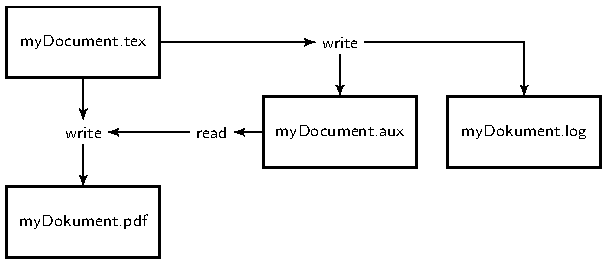
\includegraphics[width=.5\linewidth]{graphics/LaTeX-flowchart-2}
\end{center}


\section{Tables}

This is a sample text. 
\begin{tabular}[t]{llr}
	\multicolumn{2}{c}{Types of morphemes} &  \\
	\cline{1-2}
	\textbf{classification} & \textbf{type} & \textbf{example}\\
	\cline{1-2}
	form--meaning & structuralist ideal case & \emph{-st} in \emph{happiest}\\
	& portmanteau & \\
	& discontinuous & \\
	\cline{1-2}
	type of meaning & functional & \emph{whether} \\
	& lexical & \emph{table} \\
	\cline{1-2}
	dependence & free & \emph{buy} \\
	& bounded & \emph{-er}\\
%	\cline{1-2}	
%	& stem & \emph{define} \\
%	& suffix & \emph{-ing} \\
%	& prefix & \emph{pre-} \\
\end{tabular}

\blindtext 


\section{Floating environments}

\blindtext 

\begin{table}[htbp]

\centering

\begin{tabular}[t]{llr}
	\textbf{classification} & \textbf{type} & \textbf{example}\\
	\cline{1-2}
	form--meaning & structuralist ideal case & \emph{-st} in \emph{happiest}\\
	& portmanteau & \\
	& discontinuous & \\
	\cline{1-2}
	type of meaning & functional & \emph{whether} \\
	& lexical & \emph{table} \\
	\cline{1-2}
	dependence & free & \emph{buy} \\
	& bounded & \emph{-er}\\
	%	\cline{1-2}	
	%	& stem & \emph{define} \\
	%	& suffix & \emph{-ing} \\
	%	& prefix & \emph{pre-} \\
\end{tabular}

\caption{Types of morphemes}	
\end{table}


Include the file \texttt{LaTeX-flowchart-2} from the folder \texttt{graphics} into this file in a floating environment with caption. The figure should be 75\% of the line width.

\begin{figure}[htbp]
	\centering
	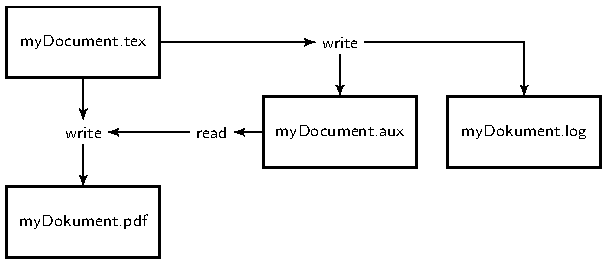
\includegraphics[width=.75\linewidth]{../../texfiles-beamer/tex-material/WissArb-latex/LaTeX-flowchart-1.pdf}
	\caption{My first float}
	\label{fig:latex-flowchart}
\end{figure}



\texttt{amssymb}

The \texttt{amssymb} package defines many math symbols 

\end{document}

%%%%%%%%%%%END DOCUMENT%%%%%%%%%%%

